\lecture{23}{12/12}

It is convenient to introduce the \textbf{Lagrangian} to the above problem:
\[ \mathcal L(x, y, \lambda) = f(x, y) + \lambda g(x, y). \]
Why? Well, suppose that $f, g$ are scalar functions in $R^2$ with 
continuous partial derivatives.
Assume the contours of $f$ are $f(x, y) = d$, as shown in Figure %todo.
\begin{figure}
    \centering
    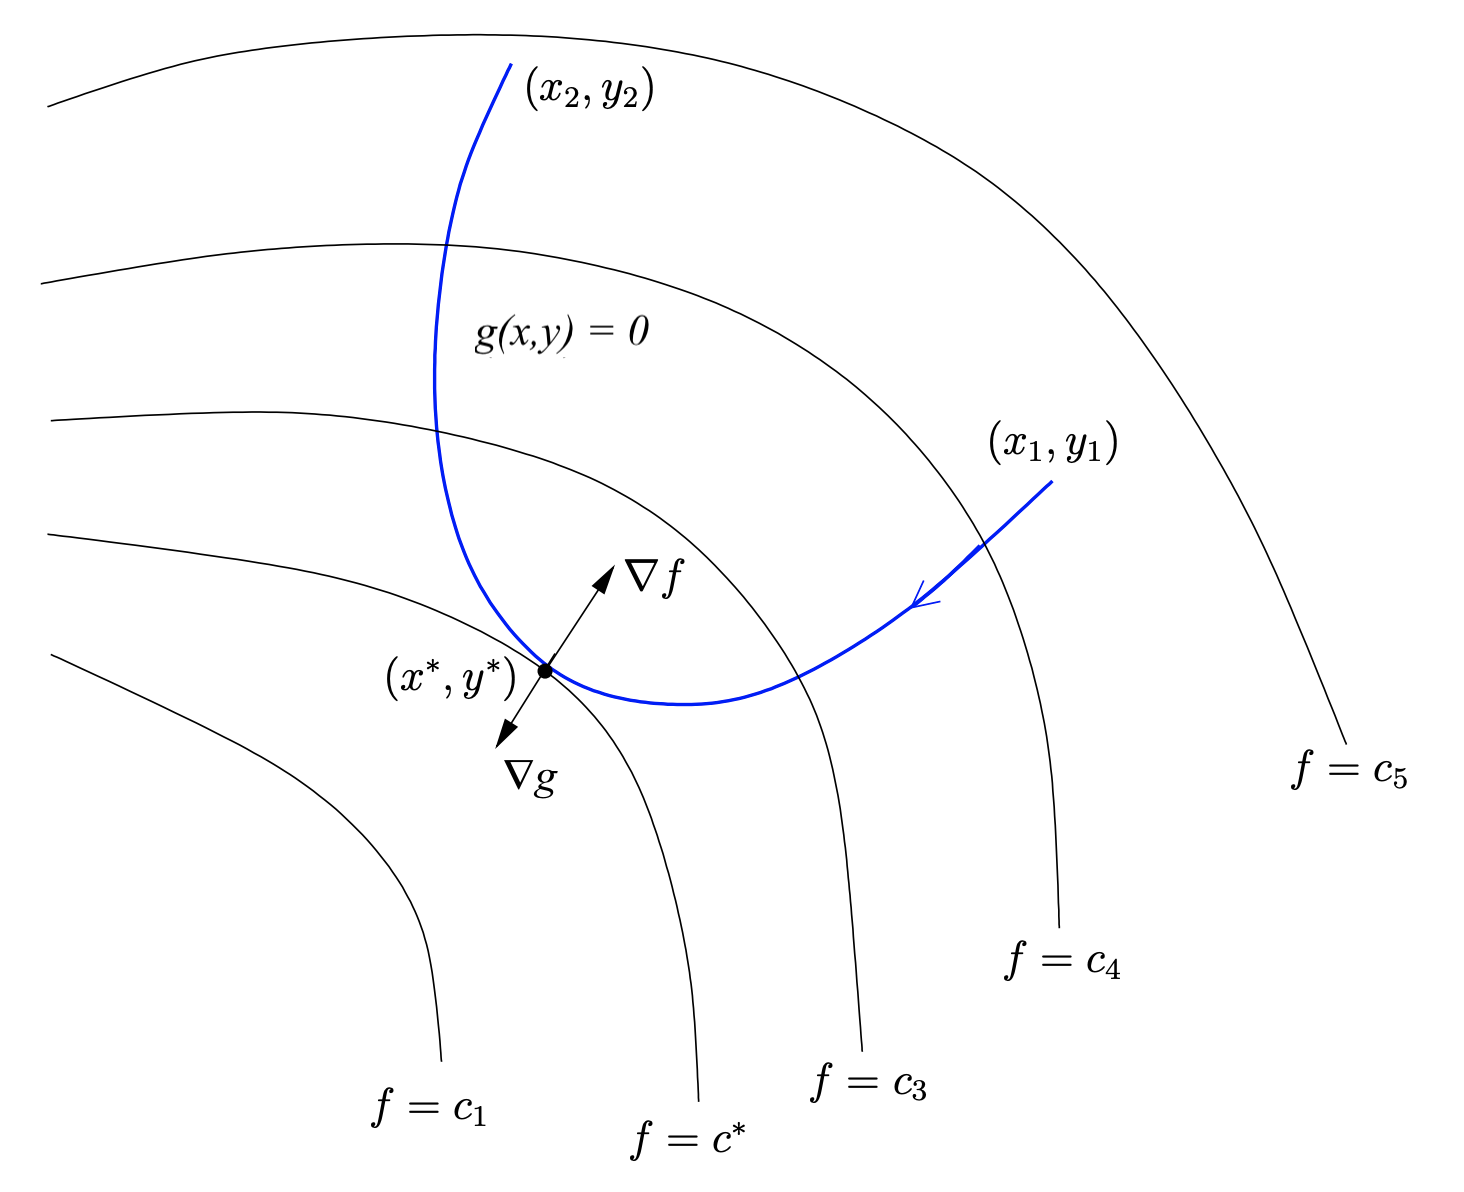
\includegraphics[width=0.7\linewidth]{images/lagrangian.png}
    \caption{The contour lines of $f$ as we move through the level set $g(x, y) = 0$.}
    \label{fig:lagrangian}
\end{figure}
As we move along the level set $g(x, y) = 0$, 
through $(x_0, y_0)$, 
the value of $f$ will be constant if either
\begin{enumerate}
    \item we are following a contour line of $f$; or
    \item $f$ is contsant anyway ($\nabla f = \bm 0$).
\end{enumerate}
Contour lines of $f$ and $g$ will be paralell at $(x_0, y_0)$ iff 
$\nabla f$ and $\nabla g$ are parallel; that is,
\[ \nabla f = \lambda \nabla g. \]
Hence, $\bm a = (x_0, y_0)$ must satisfy
\[ \nabla f(\bm a) = -\lambda\nabla g(\bm a) \qquad \text{and} \qquad
g(\bm a) = 0 \]
for some $\lambda$ known as the \textbf{Lagrange multiplier}.
This gives us \emph{stationary points}.
And so we get our expression $\mathcal L$ as above.

\begin{example}
    Find the minimum and maximum values of
    \[ f(x, y) = x + 5y \]
    on the curve $x^2 + 2y^2 = 4$.
\end{example}

\begin{solution}
    Set $g(x, y) = x^2 + y^2 - 4$.
    \[ \mathcal L(x, y, \lambda) = f(x, y) + \lambda g(x, y) =
    x + 5y + \lambda(x^2 + 2y^2 - 4). \]
    \begin{align*}
        \mathcal L_x       &= 1 + 2x\lambda = 0 \\
        \mathcal L_y       &= 5 + 4y\lambda = 0 \\
        \mathcal L_\lambda &= x^2 + y^2 - 4 = 0.
    \end{align*}
    \begin{align*}
        2y(1 + 2x\lambda) - x(5 + 4y\lambda) 
        &= 2y + 4xy\lambda - 5x - 4xy\lambda \\
        &= 2y - 5x = 0 \\ 
        x &= \frac25y \\
        \frac{4}{25}y^2 + 2y^2 - 4 &= 0 \\
        4y^2 + 50y^2 - 100 &= 0 \\
        54y^2 - 100 &= 0 \\
        y &= \pm \frac{5\sqrt2}{3\sqrt3} \\
        x &= \pm \frac{2\sqrt2}{3\sqrt3}.
    \end{align*}
    Therefore, the stationary points are
    \[ \bm a_1 = \frac{\sqrt2}{3\sqrt3}(2, 5), \qquad \bm a_2 = \frac{\sqrt2}{3\sqrt3}(-2, -5) \]
    where $\bm a_1$ is the maximum point and $\bm a_2$ is the minimum point.
\end{solution}
